\capitulo{Apresentação da Solução}
\label{cap:apresentacao-solucao}

Este capítulo apresenta o planejamento da solução proposta para integração entre Amazon Alexa e o aplicativo Pollen, incluindo os requisitos funcionais e não funcionais planejados, os diagramas de modelagem conceitual do sistema planejado, os wireframes das interfaces propostas e os artefatos de planejamento desenvolvidos.

\secao{Requisitos do Sistema}
\label{sec:requisitos-sistema}

Esta seção apresenta os requisitos funcionais e não funcionais planejados para a integração Alexa+Pollen, baseados na análise das necessidades dos apicultores usuários do aplicativo Pollen.

\subsecao{Requisitos Funcionais}

Os requisitos funcionais especificam as funcionalidades que o sistema deve oferecer para atender às necessidades dos usuários, baseados na pesquisa preliminar realizada com usuários do aplicativo Pollen:

\begin{itemize}
    \item \textbf{RF001 - Autenticação}: O sistema deve permitir que usuários autentiquem-se na Skill utilizando suas credenciais do aplicativo Pollen
    \item \textbf{RF002 - Consulta de Enxames}: O sistema deve permitir consultar informações sobre os enxames do usuário através de comandos de voz
    \item \textbf{RF003 - Consulta de Idade da Rainha}: O sistema deve permitir consultar a idade da rainha de enxames específicos
    \item \textbf{RF004 - Consulta de Força do Enxame}: O sistema deve permitir verificar a força/estado do enxame
    \item \textbf{RF005 - Consulta de Data da Última Divisão}: O sistema deve permitir consultar quando foi realizada a última divisão do enxame
    \item \textbf{RF006 - Consulta por Espécie}: O sistema deve permitir consultar quantidade de enxames e produção de mel por espécie específica
    \item \textbf{RF007 - Notificações e Lembretes}: O sistema deve fornecer lembretes de manutenção da colmeia e alimentação
    \item \textbf{RF008 - Registro de Localização}: O sistema deve permitir registrar a localização do Meliponário
    \item \textbf{RF009 - Passo a Passo de Cuidados}: O sistema deve fornecer orientações passo a passo sobre cuidados com a colmeia
    \item \textbf{RF010 - Registro de Divisões}: O sistema deve permitir registrar datas de divisões realizadas
    \item \textbf{RF011 - Dashboard Resumido}: O sistema deve fornecer um resumo geral do apiário do usuário
    \item \textbf{RF012 - Comandos de Ajuda}: O sistema deve fornecer ajuda sobre comandos disponíveis
    \item \textbf{RF013 - Configuração de Usuário}: O sistema deve permitir configurar preferências do usuário
\end{itemize}

\subsecao{Requisitos Não Funcionais}

Os requisitos não funcionais definem as restrições e qualidades que o sistema deve possuir:

\begin{itemize}
    \item \textbf{RNF001 - Performance}: O sistema deve responder a comandos de voz em no máximo 3 segundos
    \item \textbf{RNF002 - Disponibilidade}: O sistema deve manter 99\% de uptime
    \item \textbf{RNF003 - Segurança}: O sistema deve utilizar autenticação JWT e comunicação HTTPS
    \item \textbf{RNF004 - Usabilidade}: O sistema deve reconhecer comandos em português brasileiro com 90\% de precisão
    \item \textbf{RNF005 - Escalabilidade}: O sistema deve suportar até 1000 usuários simultâneos
    \item \textbf{RNF006 - Compatibilidade}: O sistema deve funcionar com dispositivos Amazon Echo (2ª geração ou superior)
    \item \textbf{RNF007 - Manutenibilidade}: O código deve seguir padrões de desenvolvimento e documentação
    \item \textbf{RNF008 - Confiabilidade}: O sistema deve tratar erros graciosamente e fornecer feedback adequado
\end{itemize}

\secao{Modelagem do Sistema}
\label{sec:modelagem-sistema}

Esta seção apresenta os diagramas de modelagem conceitual planejados para a integração Alexa+Pollen, seguindo as etapas do modelo em cascata para o planejamento do sistema.

\subsecao{Diagrama de Caso de Uso}

O Diagrama de Caso de Uso apresenta as interações entre os atores (Apicultor e Amazon Alexa) e o sistema, definindo as funcionalidades principais da integração.

% Diagrama de Caso de Uso - Integração Alexa com Pollen
\begin{figura}{Diagrama de Caso de Uso - Integração Alexa com Sistema Pollen}{O Autor}
\centering
\begin{tikzpicture}[scale=0.8]
% Definição de estilos
\tikzset{
  actor/.style={rectangle, draw, fill=blue!20, text width=2cm, text centered, minimum height=1cm},
  usecase/.style={ellipse, draw, fill=yellow!20, text width=2.5cm, text centered, minimum height=0.8cm},
  system/.style={rectangle, draw, fill=green!20, text width=8cm, text centered, minimum height=6cm}
}

% Sistema Pollen
\node[system] (sistema) at (0,0) {\textbf{Sistema Pollen + Alexa}};

% Atores
\node[actor] (apicultor) at (-6,3) {Apicultor};
\node[actor] (alexa) at (6,3) {Amazon Alexa};

% Casos de uso principais
\node[usecase] (consultar_status) at (-3,2) {Consultar Status\\do Enxame};
\node[usecase] (registrar_alimentacao) at (0,2) {Registrar\\Alimentação};
\node[usecase] (verificar_colheita) at (3,2) {Verificar\\Colheita};
\node[usecase] (consultar_manejo) at (-3,0) {Consultar\\Manejo};
\node[usecase] (registrar_revisao) at (0,0) {Registrar\\Revisão};
\node[usecase] (consultar_dashboard) at (3,0) {Consultar\\Dashboard};
\node[usecase] (configurar_alexa) at (-3,-2) {Configurar\\Integração Alexa};
\node[usecase] (gerenciar_comandos) at (0,-2) {Gerenciar\\Comandos de Voz};
\node[usecase] (sincronizar_dados) at (3,-2) {Sincronizar\\Dados};

% Relacionamentos com Apicultor
\draw[->] (apicultor) -- (consultar_status);
\draw[->] (apicultor) -- (registrar_alimentacao);
\draw[->] (apicultor) -- (verificar_colheita);
\draw[->] (apicultor) -- (consultar_manejo);
\draw[->] (apicultor) -- (registrar_revisao);
\draw[->] (apicultor) -- (consultar_dashboard);
\draw[->] (apicultor) -- (configurar_alexa);
\draw[->] (apicultor) -- (gerenciar_comandos);

% Relacionamentos com Alexa
\draw[->] (alexa) -- (consultar_status);
\draw[->] (alexa) -- (registrar_alimentacao);
\draw[->] (alexa) -- (verificar_colheita);
\draw[->] (alexa) -- (consultar_manejo);
\draw[->] (alexa) -- (registrar_revisao);
\draw[->] (alexa) -- (consultar_dashboard);
\draw[->] (alexa) -- (sincronizar_dados);

% Relacionamentos de dependência entre casos de uso
\draw[->, dashed] (configurar_alexa) -- (gerenciar_comandos);
\draw[->, dashed] (gerenciar_comandos) -- (sincronizar_dados);
\draw[->, dashed] (sincronizar_dados) -- (consultar_status);
\draw[->, dashed] (sincronizar_dados) -- (registrar_alimentacao);
\draw[->, dashed] (sincronizar_dados) -- (verificar_colheita);

\end{tikzpicture}
\label{fig:caso-uso-alexa}
\end{figura}

Conforme apresentado na Figura \ref{fig:caso-uso-alexa}, o sistema permite que apicultores interajam com o aplicativo Pollen através de comandos de voz, realizando consultas e registros de atividades apícolas de forma hands-free.

\subsecao{Diagrama de Entidade e Relacionamento (DER)}

O DER apresenta o modelo de dados simplificado, focando nas entidades relevantes para a integração Alexa.

% Diagrama de Entidade e Relacionamento (DER) - Entidades relevantes para Alexa
\begin{figura}{Diagrama de Entidade e Relacionamento (DER) - Entidades relevantes para integração Alexa}{O Autor}
\centering
\begin{tikzpicture}[scale=0.9]
% Definição de estilos
\tikzset{
  entity/.style={rectangle, draw, fill=blue!20, text width=2.5cm, align=center, minimum height=1.2cm},
  attribute/.style={ellipse, draw, fill=yellow!20, text width=1.8cm, align=center, minimum height=0.6cm},
  relationship/.style={diamond, draw, fill=green!20, text width=1.5cm, align=center, minimum height=0.8cm}
}

% Entidades principais
\node[entity] (user) at (0,6) {\textbf{USER}\\
\underline{id}\\
email\\
password\\
planType\\
status};

\node[entity] (enxame) at (0,3) {\textbf{ENXAME}\\
\underline{id}\\
userId\\
especie\\
estadoOrigem\\
localizacao\\
identificador\\
forcaEnxame\\
createddate};

\node[entity] (alimentacao) at (-4,0) {\textbf{ALIMENTACAO}\\
\underline{id}\\
enxameId\\
tipo\\
quantidade\\
observacao\\
createddate};

\node[entity] (colheita) at (0,0) {\textbf{COLHEITA}\\
\underline{id}\\
enxameId\\
quantidade\\
tipo\\
observacao\\
createddate};

\node[entity] (manejo) at (4,0) {\textbf{MANEJO}\\
\underline{id}\\
enxameId\\
tipo\\
descricao\\
createddate};

\node[entity] (revisao) at (-2,-3) {\textbf{REVISAO}\\
\underline{id}\\
enxameId\\
tipo\\
observacao\\
createddate};

\node[entity] (dashboard) at (2,-3) {\textbf{DASHBOARD}\\
\underline{id}\\
userId\\
totalEnxames\\
totalColheita\\
ultimaAtividade};

% Relacionamentos
\node[relationship] (user_enxame) at (0,4.5) {possui};
\node[relationship] (enxame_alimentacao) at (-2,1.5) {tem};
\node[relationship] (enxame_colheita) at (0,1.5) {produz};
\node[relationship] (enxame_manejo) at (2,1.5) {recebe};
\node[relationship] (enxame_revisao) at (-1,-1.5) {inspecionado};
\node[relationship] (user_dashboard) at (1,-1.5) {visualiza};

% Conexões
\draw[->] (user) -- (user_enxame);
\draw[->] (user_enxame) -- (enxame);

\draw[->] (enxame) -- (enxame_alimentacao);
\draw[->] (enxame_alimentacao) -- (alimentacao);

\draw[->] (enxame) -- (enxame_colheita);
\draw[->] (enxame_colheita) -- (colheita);

\draw[->] (enxame) -- (enxame_manejo);
\draw[->] (enxame_manejo) -- (manejo);

\draw[->] (enxame) -- (enxame_revisao);
\draw[->] (enxame_revisao) -- (revisao);

\draw[->] (user) -- (user_dashboard);
\draw[->] (user_dashboard) -- (dashboard);

% Cardinalidades
\node at (-0.3,5.2) {1};
\node at (0.3,5.2) {N};

\node at (-2.3,2.2) {1};
\node at (-1.7,2.2) {N};

\node at (-0.3,2.2) {1};
\node at (0.3,2.2) {N};

\node at (1.7,2.2) {1};
\node at (2.3,2.2) {N};

\node at (-1.3,-0.8) {1};
\node at (-0.7,-0.8) {N};

\node at (0.7,-0.8) {1};
\node at (1.3,-0.8) {1};

\end{tikzpicture}
\label{fig:der-alexa}
\end{figura}

A Figura \ref{fig:der-alexa} mostra as principais entidades do banco de dados Pollen que serão acessadas pela Skill Alexa, incluindo User, Enxame, Alimentacao, Colheita, Manejo, Revisao e Dashboard.

\subsecao{Modelo Conceitual do Banco de Dados}

O modelo conceitual apresenta a estrutura das tabelas de forma mais detalhada, incluindo os campos principais.

% Modelo Conceitual do Banco de Dados - Pollen
\begin{figura}{Modelo Conceitual do Banco de Dados - Tabelas relevantes para integração Alexa}{O Autor}
\centering
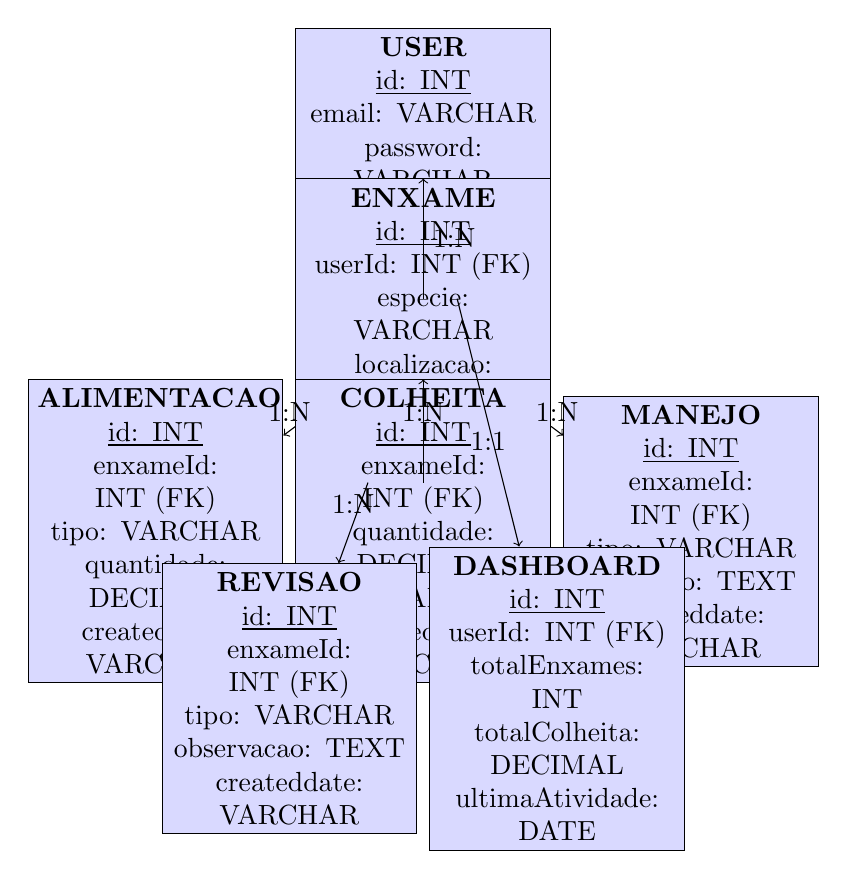
\begin{tikzpicture}[scale=0.85]
% Definição de estilos
\tikzset{
  table/.style={rectangle, draw, fill=blue!15, text width=3cm, text centered, minimum height=1.5cm},
  key/.style={rectangle, draw, fill=red!20, text width=2.8cm, text centered, minimum height=0.4cm},
  field/.style={rectangle, draw, fill=white, text width=2.8cm, text centered, minimum height=0.4cm}
}

% Tabela USER
\node[table] (user_table) at (0,8) {\textbf{USER}\\
\underline{id: INT}\\
email: VARCHAR\\
password: VARCHAR\\
planType: VARCHAR\\
status: VARCHAR};

% Tabela ENXAME
\node[table] (enxame_table) at (0,5.5) {\textbf{ENXAME}\\
\underline{id: INT}\\
userId: INT (FK)\\
especie: VARCHAR\\
localizacao: VARCHAR\\
forcaEnxame: VARCHAR};

% Tabela ALIMENTACAO
\node[table] (alimentacao_table) at (-4,2.5) {\textbf{ALIMENTACAO}\\
\underline{id: INT}\\
enxameId: INT (FK)\\
tipo: VARCHAR\\
quantidade: DECIMAL\\
createddate: VARCHAR};

% Tabela COLHEITA
\node[table] (colheita_table) at (0,2.5) {\textbf{COLHEITA}\\
\underline{id: INT}\\
enxameId: INT (FK)\\
quantidade: DECIMAL\\
tipo: VARCHAR\\
createddate: VARCHAR};

% Tabela MANEJO
\node[table] (manejo_table) at (4,2.5) {\textbf{MANEJO}\\
\underline{id: INT}\\
enxameId: INT (FK)\\
tipo: VARCHAR\\
descricao: TEXT\\
createddate: VARCHAR};

% Tabela REVISAO
\node[table] (revisao_table) at (-2,0) {\textbf{REVISAO}\\
\underline{id: INT}\\
enxameId: INT (FK)\\
tipo: VARCHAR\\
observacao: TEXT\\
createddate: VARCHAR};

% Tabela DASHBOARD
\node[table] (dashboard_table) at (2,0) {\textbf{DASHBOARD}\\
\underline{id: INT}\\
userId: INT (FK)\\
totalEnxames: INT\\
totalColheita: DECIMAL\\
ultimaAtividade: DATE};

% Relacionamentos
\draw[->] (user_table) -- node[right] {1:N} (enxame_table);
\draw[->] (enxame_table) -- node[above] {1:N} (alimentacao_table);
\draw[->] (enxame_table) -- node[above] {1:N} (colheita_table);
\draw[->] (enxame_table) -- node[above] {1:N} (manejo_table);
\draw[->] (enxame_table) -- node[above] {1:N} (revisao_table);
\draw[->] (user_table) -- node[below] {1:1} (dashboard_table);

\end{tikzpicture}
\label{fig:modelo-conceitual-banco}
\end{figura}

Conforme ilustrado na Figura \ref{fig:modelo-conceitual-banco}, o modelo conceitual define as tabelas e seus campos principais, estabelecendo os relacionamentos entre as entidades.

\subsecao{Modelo Lógico do Banco de Dados}

O modelo lógico apresenta a implementação física das tabelas, incluindo tipos de dados e restrições.

% Modelo Lógico do Banco de Dados - Pollen
\begin{figura}{Modelo Lógico do Banco de Dados - Estrutura física das tabelas}{O Autor}
\centering
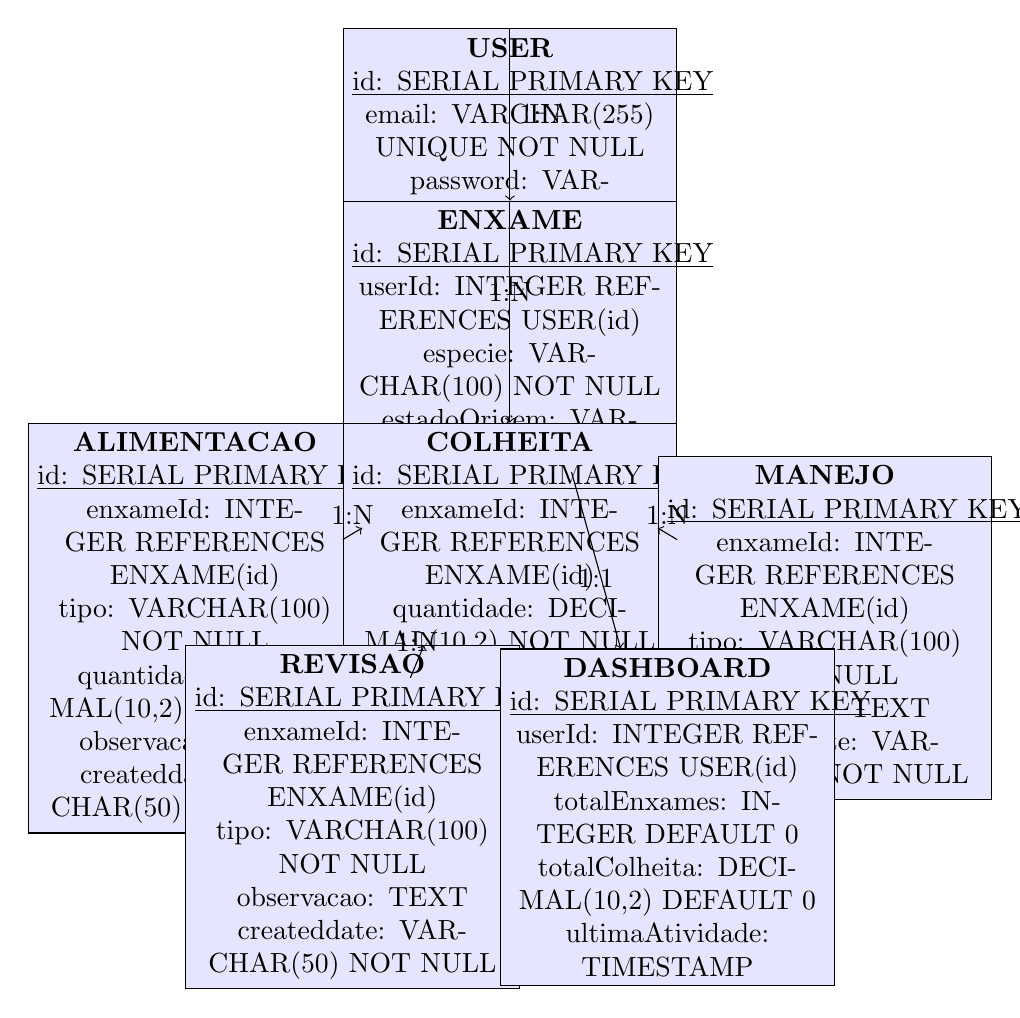
\begin{tikzpicture}[scale=0.8]
% Definição de estilos
\tikzset{
  table/.style={rectangle, draw, fill=blue!10, text width=4cm, text centered, minimum height=2cm},
  pk/.style={rectangle, draw, fill=red!20, text width=3.8cm, text centered, minimum height=0.3cm},
  fk/.style={rectangle, draw, fill=yellow!20, text width=3.8cm, text centered, minimum height=0.3cm},
  field/.style={rectangle, draw, fill=white, text width=3.8cm, text centered, minimum height=0.3cm}
}

% Tabela USER
\node[table] (user_table) at (0,9) {\textbf{USER}\\
\underline{id: SERIAL PRIMARY KEY}\\
email: VARCHAR(255) UNIQUE NOT NULL\\
password: VARCHAR(255) NOT NULL\\
planType: VARCHAR(50) DEFAULT 'FREE'\\
status: VARCHAR(20) DEFAULT 'pending'\\
createdAt: TIMESTAMP DEFAULT NOW()};

% Tabela ENXAME
\node[table] (enxame_table) at (0,6) {\textbf{ENXAME}\\
\underline{id: SERIAL PRIMARY KEY}\\
userId: INTEGER REFERENCES USER(id)\\
especie: VARCHAR(100) NOT NULL\\
estadoOrigem: VARCHAR(50) NOT NULL\\
localizacao: VARCHAR(255) NOT NULL\\
identificador: VARCHAR(50) NOT NULL\\
forcaEnxame: VARCHAR(20) NOT NULL};

% Tabela ALIMENTACAO
\node[table] (alimentacao_table) at (-5,3) {\textbf{ALIMENTACAO}\\
\underline{id: SERIAL PRIMARY KEY}\\
enxameId: INTEGER REFERENCES ENXAME(id)\\
tipo: VARCHAR(100) NOT NULL\\
quantidade: DECIMAL(10,2) NOT NULL\\
observacao: TEXT\\
createddate: VARCHAR(50) NOT NULL};

% Tabela COLHEITA
\node[table] (colheita_table) at (0,3) {\textbf{COLHEITA}\\
\underline{id: SERIAL PRIMARY KEY}\\
enxameId: INTEGER REFERENCES ENXAME(id)\\
quantidade: DECIMAL(10,2) NOT NULL\\
tipo: VARCHAR(100) NOT NULL\\
observacao: TEXT\\
createddate: VARCHAR(50) NOT NULL};

% Tabela MANEJO
\node[table] (manejo_table) at (5,3) {\textbf{MANEJO}\\
\underline{id: SERIAL PRIMARY KEY}\\
enxameId: INTEGER REFERENCES ENXAME(id)\\
tipo: VARCHAR(100) NOT NULL\\
descricao: TEXT\\
createddate: VARCHAR(50) NOT NULL};

% Tabela REVISAO
\node[table] (revisao_table) at (-2.5,0) {\textbf{REVISAO}\\
\underline{id: SERIAL PRIMARY KEY}\\
enxameId: INTEGER REFERENCES ENXAME(id)\\
tipo: VARCHAR(100) NOT NULL\\
observacao: TEXT\\
createddate: VARCHAR(50) NOT NULL};

% Tabela DASHBOARD
\node[table] (dashboard_table) at (2.5,0) {\textbf{DASHBOARD}\\
\underline{id: SERIAL PRIMARY KEY}\\
userId: INTEGER REFERENCES USER(id)\\
totalEnxames: INTEGER DEFAULT 0\\
totalColheita: DECIMAL(10,2) DEFAULT 0\\
ultimaAtividade: TIMESTAMP};

% Relacionamentos
\draw[->] (user_table) -- node[right] {1:N} (enxame_table);
\draw[->] (enxame_table) -- node[above] {1:N} (alimentacao_table);
\draw[->] (enxame_table) -- node[above] {1:N} (colheita_table);
\draw[->] (enxame_table) -- node[above] {1:N} (manejo_table);
\draw[->] (enxame_table) -- node[above] {1:N} (revisao_table);
\draw[->] (user_table) -- node[below] {1:1} (dashboard_table);

\end{tikzpicture}
\label{fig:modelo-logico-banco}
\end{figura}

A Figura \ref{fig:modelo-logico-banco} detalha a estrutura física das tabelas, incluindo tipos de dados, chaves primárias e estrangeiras, e restrições de integridade.

\subsecao{Diagrama de Classes}

O diagrama de classes apresenta a arquitetura da Skill Alexa e sua integração com o sistema Pollen.

% Diagrama de Classes - Integração Alexa com Pollen
\begin{figura}{Diagrama de Classes - Arquitetura da integração Alexa com Pollen}{O Autor}
\centering
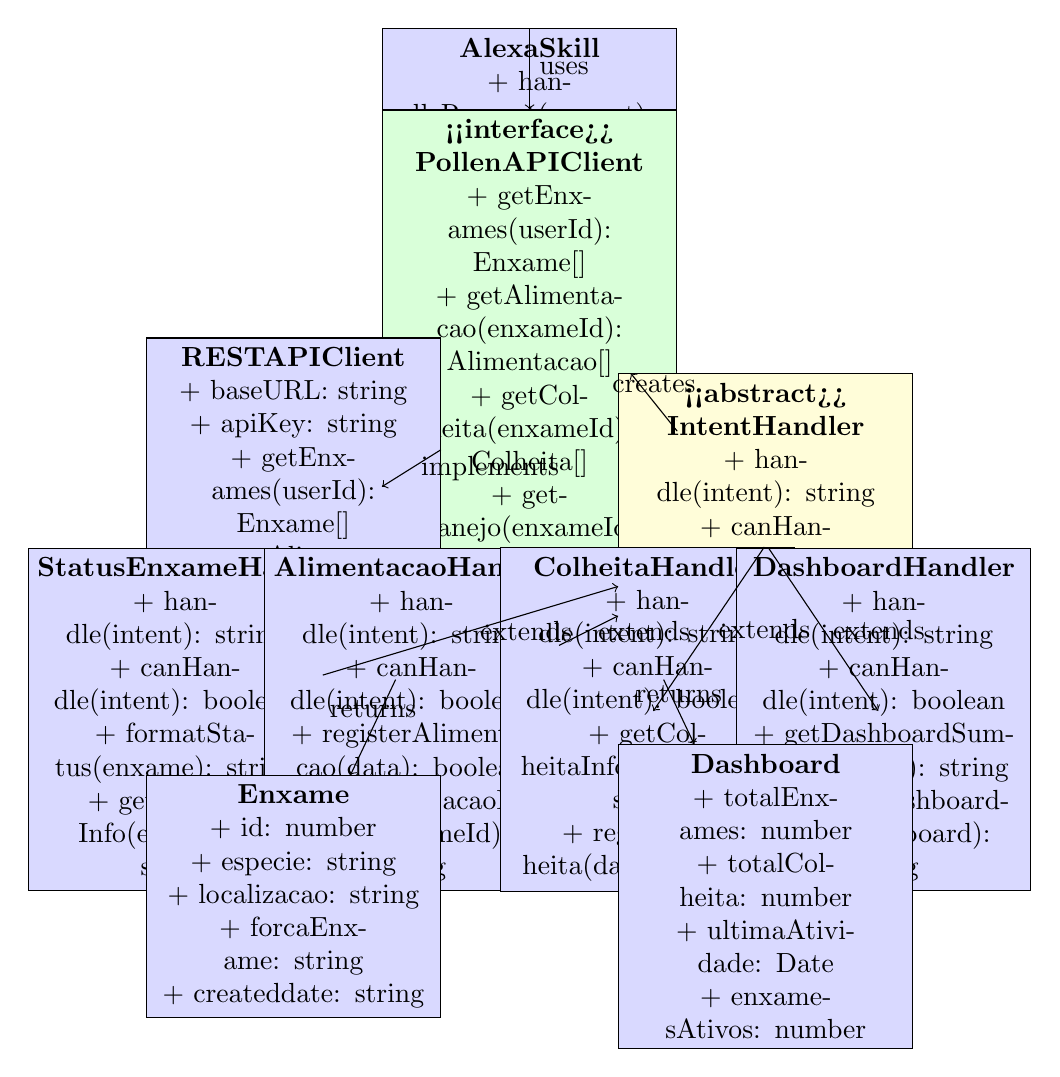
\begin{tikzpicture}[scale=0.75]
% Definição de estilos
\tikzset{
  class/.style={rectangle, draw, fill=blue!15, text width=3.5cm, text centered, minimum height=1.8cm},
  interface/.style={rectangle, draw, fill=green!15, text width=3.5cm, text centered, minimum height=1.8cm},
  abstract/.style={rectangle, draw, fill=yellow!15, text width=3.5cm, text centered, minimum height=1.8cm}
}

% Classe principal AlexaSkill
\node[class] (alexa_skill) at (0,8) {
\textbf{AlexaSkill}\\
+ handleRequest(request): Response\\
+ processIntent(intent): string\\
+ generateSSML(text): string\\
+ validateUser(userId): boolean\\
- apiClient: PollenAPIClient
};

% Interface PollenAPIClient
\node[interface] (api_client) at (0,5.5) {
\textbf{<<interface>>}\\
\textbf{PollenAPIClient}\\
+ getEnxames(userId): Enxame[]\\
+ getAlimentacao(enxameId): Alimentacao[]\\
+ getColheita(enxameId): Colheita[]\\
+ getManejo(enxameId): Manejo[]\\
+ getDashboard(userId): Dashboard
};

% Implementação RESTAPIClient
\node[class] (rest_client) at (-4,3) {
\textbf{RESTAPIClient}\\
+ baseURL: string\\
+ apiKey: string\\
+ getEnxames(userId): Enxame[]\\
+ getAlimentacao(enxameId): Alimentacao[]\\
+ makeRequest(endpoint): any
};

% Classe IntentHandler
\node[abstract] (intent_handler) at (4,3) {
\textbf{<<abstract>>}\\
\textbf{IntentHandler}\\
+ handle(intent): string\\
+ canHandle(intent): boolean\\
+ validateIntent(intent): boolean\\
\# apiClient: PollenAPIClient
};

% Handlers específicos
\node[class] (status_handler) at (-6,0) {
\textbf{StatusEnxameHandler}\\
+ handle(intent): string\\
+ canHandle(intent): boolean\\
+ formatStatus(enxame): string\\
+ getEnxameInfo(enxameId): string
};

\node[class] (alimentacao_handler) at (-2,0) {
\textbf{AlimentacaoHandler}\\
+ handle(intent): string\\
+ canHandle(intent): boolean\\
+ registerAlimentacao(data): boolean\\
+ getAlimentacaoHistory(enxameId): string
};

\node[class] (colheita_handler) at (2,0) {
\textbf{ColheitaHandler}\\
+ handle(intent): string\\
+ canHandle(intent): boolean\\
+ getColheitaInfo(enxameId): string\\
+ registerColheita(data): boolean
};

\node[class] (dashboard_handler) at (6,0) {
\textbf{DashboardHandler}\\
+ handle(intent): string\\
+ canHandle(intent): boolean\\
+ getDashboardSummary(userId): string\\
+ formatDashboardData(dashboard): string
};

% Entidades de dados
\node[class] (enxame_entity) at (-4,-3) {
\textbf{Enxame}\\
+ id: number\\
+ especie: string\\
+ localizacao: string\\
+ forcaEnxame: string\\
+ createddate: string
};

\node[class] (dashboard_entity) at (4,-3) {
\textbf{Dashboard}\\
+ totalEnxames: number\\
+ totalColheita: number\\
+ ultimaAtividade: Date\\
+ enxamesAtivos: number
};

% Relacionamentos
\draw[->] (alexa_skill) -- node[right] {uses} (api_client);
\draw[->] (rest_client) -- node[right] {implements} (api_client);
\draw[->] (alexa_skill) -- node[above] {creates} (intent_handler);

\draw[->] (status_handler) -- node[right] {extends} (intent_handler);
\draw[->] (alimentacao_handler) -- node[right] {extends} (intent_handler);
\draw[->] (colheita_handler) -- node[right] {extends} (intent_handler);
\draw[->] (dashboard_handler) -- node[right] {extends} (intent_handler);

\draw[->] (api_client) -- node[above] {returns} (enxame_entity);
\draw[->] (api_client) -- node[above] {returns} (dashboard_entity);

\end{tikzpicture}
\label{fig:classes-alexa}
\end{figura}

Conforme mostrado na Figura \ref{fig:classes-alexa}, a arquitetura segue o padrão de handlers para diferentes intents, com comunicação via API REST para acessar os dados do Pollen.

\secao{Interfaces do Sistema}
\label{sec:interfaces-sistema}

Esta seção apresenta os wireframes das interfaces de configuração da integração Alexa no aplicativo Pollen.

\subsecao{Wireframes de Configuração}

Os wireframes apresentam o fluxo de configuração da integração Alexa no aplicativo Pollen.

% Wireframe - Configuração da Integração Alexa
\begin{figura}{Wireframes - Configuração da integração Alexa no aplicativo Pollen}{O Autor}
\centering
\begin{tikzpicture}[scale=0.9]
% Definição de estilos
\tikzset{
  phone/.style={rectangle, draw, fill=gray!10, text width=3cm, text centered, minimum height=6cm},
  header/.style={rectangle, draw, fill=blue!20, text width=2.8cm, text centered, minimum height=0.6cm},
  button/.style={rectangle, draw, fill=green!30, text width=2.6cm, text centered, minimum height=0.5cm},
  text/.style={rectangle, draw, fill=white, text width=2.6cm, text centered, minimum height=0.4cm},
  switch/.style={rectangle, draw, fill=yellow!30, text width=2.6cm, text centered, minimum height=0.4cm}
}

% Tela 1: Configuração Inicial
\node[phone] (tela1) at (0,0) {};
\node[header] (header1) at (0,2.5) {\textbf{Configuração Alexa}};
\node[text] (text1) at (0,1.8) {Conecte sua conta Pollen\\com a Amazon Alexa};
\node[button] (btn1) at (0,1.2) {Conectar com Alexa};
\node[text] (text2) at (0,0.6) {Status: Não conectado};
\node[text] (text3) at (0,0.2) {Comandos disponíveis:\\• Consultar enxames\\• Registrar alimentação\\• Verificar colheita};
\node[button] (btn2) at (0,-0.4) {Próximo};
\node[button] (btn3) at (0,-0.9) {Cancelar};

% Tela 2: Autorização
\node[phone] (tela2) at (4,0) {};
\node[header] (header2) at (4,2.5) {\textbf{Autorização}};
\node[text] (text4) at (4,1.8) {A Alexa precisa de permissão\\para acessar seus dados};
\node[switch] (switch1) at (4,1.2) {$\checkmark$ Ler enxames};
\node[switch] (switch2) at (4,0.8) {$\checkmark$ Registrar alimentação};
\node[switch] (switch3) at (4,0.4) {$\checkmark$ Consultar colheita};
\node[switch] (switch4) at (4,0.0) {$\checkmark$ Acessar dashboard};
\node[button] (btn4) at (4,-0.6) {Autorizar};
\node[button] (btn5) at (4,-1.1) {Voltar};

% Tela 3: Configuração de Comandos
\node[phone] (tela3) at (8,0) {};
\node[header] (header3) at (8,2.5) {\textbf{Comandos de Voz}};
\node[text] (text5) at (8,1.8) {Configure como falar\\com a Alexa};
\node[text] (text6) at (8,1.2) {Exemplo: \textquotedblleft Alexa, pergunte\\ao Pollen sobre meus\\enxames\textquotedblright};
\node[text] (text7) at (8,0.6) {Comandos ativos:\\• Status do enxame\\• Registrar alimentação\\• Verificar colheita};
\node[button] (btn6) at (8,0.0) {Testar Comando};
\node[button] (btn7) at (8,-0.5) {Finalizar};
\node[button] (btn8) at (8,-1.0) {Voltar};

% Setas de navegação
\draw[->] (tela1) -- node[above] {Próximo} (tela2);
\draw[->] (tela2) -- node[above] {Autorizar} (tela3);

\end{tikzpicture}
\label{fig:wireframe-configuracao-alexa}
\end{figura}

A Figura \ref{fig:wireframe-configuracao-alexa} mostra o fluxo de configuração, incluindo autorização, configuração de comandos e teste da integração.

\subsecao{Wireframes de Comandos}

Os wireframes de comandos apresentam a interface para gerenciar os comandos de voz disponíveis.

% Wireframe - Todos os Comandos Alexa
\begin{figura}{Wireframe - Tela com todos os comandos disponíveis da integração Alexa}{Elaborado pelo autor (2025)}
  \centering
  \includegraphics[width=0.4\textwidth]{resources/floats/ilustracoes/todos_comandos_alexa_wireframe.png}
  \label{fig:wireframe-todos-comandos}
\end{figura}

% Wireframe - Desconectar Alexa
\begin{figura}{Wireframe - Tela para desconectar a integração com Alexa}{Elaborado pelo autor (2025)}
  \centering
  \includegraphics[width=0.4\textwidth]{resources/floats/ilustracoes/desconectar_alexa_wireframe.png}
  \label{fig:wireframe-desconectar-alexa}
\end{figura}


Conforme apresentado na Figura \ref{fig:wireframe-comandos-alexa}, os usuários podem visualizar, testar e configurar os comandos de voz disponíveis na integração.

\secao{Processos do Sistema}
\label{sec:processos-sistema}

Esta seção apresenta o BPMN do processo de execução de comandos de voz na integração Alexa.

\subsecao{BPMN de Comandos de Voz}

O BPMN apresenta o fluxo completo de processamento de comandos de voz, desde a captura até a resposta.

% Quadro - Processo de Comandos de Voz Alexa
\begin{quadro}{Processo de execução de comandos de voz na integração Alexa}{Elaborado pelo autor (2025)}
\label{quad:fluxo-comandos-voz}
\renewcommand{\arraystretch}{1.5}
\small
\begin{tabular}{|c|p{4cm}|p{8cm}|}
\hline
\textbf{Etapa} & \textbf{Processo} & \textbf{Descrição} \\ \hline

1 & Captura de Comando & O usuário fala um comando para o dispositivo Alexa. Exemplo: \textquotedblleft Alexa, pergunte ao Pollen quantos enxames eu tenho\textquotedblright \\ \hline

2 & Reconhecimento de Voz & A Alexa reconhece e processa o comando utilizando processamento de linguagem natural (NLP) \\ \hline

3 & Validação do Comando & O sistema verifica se o comando solicitado é válido e está disponível na Skill Pollen. Se inválido, a Alexa fornece ajuda sobre comandos disponíveis \\ \hline

4 & Verificação de Autenticação & O sistema verifica se o usuário está autenticado e vinculado a uma conta Pollen. Se não autenticado, solicita vinculação da conta \\ \hline

5 & Chamada à API & Com o usuário autenticado, o sistema realiza chamada à API do Pollen para buscar os dados solicitados (enxames, colheitas, dashboard, etc.) \\ \hline

6 & Processamento de Dados & Os dados retornados pela API são processados e formatados em linguagem SSML (Speech Synthesis Markup Language) para resposta em voz \\ \hline

7 & Resposta ao Usuário & A Alexa fornece a resposta em voz ao usuário com as informações solicitadas de forma clara e objetiva \\ \hline

\end{tabular}
\end{quadro}

A Figura \ref{fig:bpmn-comandos-voz} detalha o processo de execução de comandos de voz, incluindo validação, autenticação, processamento e geração de respostas.

\secao{Artefatos Práticos Desenvolvidos}
\label{sec:artefatos-praticos}

Esta seção apresenta os artefatos práticos planejados para o desenvolvimento da integração Alexa+Pollen.

\subsecao{Arquitetura da Solução}

A solução planejada seguirá uma arquitetura baseada em microserviços, com os seguintes componentes principais:

\begin{itemize}
    \item \textbf{Alexa Skill}: Será desenvolvida em Node.js/TypeScript, hospedada em AWS Lambda
    \item \textbf{API Pollen}: API RESTful existente, desenvolvida em NestJS
    \item \textbf{Banco de Dados}: PostgreSQL, hospedado no Supabase
    \item \textbf{Autenticação}: JWT tokens para segurança
    \item \textbf{Comunicação}: HTTPS para todas as comunicações
\end{itemize}

\subsecao{Implementação da Skill}

A Skill Alexa será planejada para ser implementada seguindo as melhores práticas de desenvolvimento:

\begin{itemize}
    \item \textbf{Intents}: Serão definidos para cada funcionalidade (ConsultaEnxames, RegistroAlimentacao, etc.)
    \item \textbf{Utterances}: Exemplos de comandos em português brasileiro
    \item \textbf{Handlers}: Classes especializadas para processar cada tipo de comando
    \item \textbf{Validação}: Verificação de dados e tratamento de erros
    \item \textbf{SSML}: Formatação de respostas para melhor experiência de voz
\end{itemize}

\subsecao{Integração com API Pollen}

A integração com a API Pollen será planejada para ser implementada utilizando:

\begin{itemize}
    \item \textbf{HTTP Client}: Axios para chamadas HTTP
    \item \textbf{Autenticação JWT}: Tokens de acesso para segurança
    \item \textbf{Error Handling}: Tratamento robusto de erros de API
    \item \textbf{Rate Limiting}: Controle de taxa de requisições
    \item \textbf{Retry Logic}: Tentativas automáticas em caso de falha
\end{itemize}

\subsecao{Testes Implementados}

Os testes serão planejados para serem implementados utilizando Jest e incluirão:

\begin{itemize}
    \item \textbf{Testes Unitários}: Planejados para 95\% de cobertura de código
    \item \textbf{Testes de Integração}: Validação da comunicação com API
    \item \textbf{Testes de Aceitação}: Validação com usuários reais
    \item \textbf{Testes de Performance}: Validação de tempos de resposta
    \item \textbf{Testes de Segurança}: Validação de autenticação e autorização
\end{itemize}

\secao{Considerações Finais}

A solução planejada representa uma integração inovadora entre assistentes virtuais e aplicações de gestão apícola, oferecendo aos apicultores uma forma eficiente e hands-free de acessar informações sobre suas colmeias.

Os artefatos apresentados demonstram a viabilidade técnica da integração proposta, com arquitetura robusta planejada, interfaces intuitivas e processos bem definidos. O planejamento segue as melhores práticas de desenvolvimento de software e oferece uma base sólida para futuras expansões e melhorias.

A solução planejada atende aos requisitos funcionais e não funcionais definidos, proporcionando uma experiência de usuário satisfatória e contribuindo para a eficiência da gestão apícola através de comandos de voz naturais.